\documentclass[a4paper,french,12pt]{article}
\usepackage[french]{babel}
\usepackage[utf8]{inputenc}
\usepackage{float}
\usepackage{amsmath}
\usepackage{graphicx}
\usepackage{url}
\usepackage{hyperref}
\usepackage{setspace}
\usepackage{abstract}
\usepackage[T1]{fontenc}
\usepackage[top=2cm, bottom=2.5cm, left=2.5cm, right=2.5cm]{geometry}\pagestyle{plain}
\usepackage{subfig}
\usepackage[bottom]{footmisc}
\usepackage{pdfpages}
\usepackage{titlesec}
\usepackage{perpage}

\title{Rapport Stage 1A}
\author{Adib Habbou}
\date{May 2022}

\begin{document}

\begin{titlepage}
\begin{center}

\includegraphics[height=5cm]{ENSIIE.png}~\\[1.2cm]

{\large École Nationale Supérieure d'Informatique pour l'Industrie et l'Entreprise\\[1.0cm]}

\HRule \\[0.5cm]

{\huge \bfseries Rapport de stage\\[0.6cm]}
{\Large \bfseries « Développement d'une application pour le Web-Scraping et l'analyse des données textuelles »\\[0.5cm] }

\HRule \\[1.0cm]

{\large
\emph{Étudiant} : \textbf{Adib HABBOU}\\[0.3cm]
\emph{Tuteur académique à l'ENSIIE} : \textbf{Nicolas BRUNEL}\\

\HRule \\[1.0cm]

\includegraphics[height=5cm]{HCP.png}~\\[0.5cm]

\HRule \\[0.5cm]

\emph{Établissement} : \textbf{Haut-Commissariat au Plan} (Rabat, Maroc)\\[0.3cm]
\emph{Maître de stage} : \textbf{Oumaima HOURRANE}\\}

\vfill

\vspace*{1.0cm}{\normalsize{Stage de première année du lundi 23 mai 2022 au vendredi 15 juillet 2022}}

\end{center}
\end{titlepage}

\section*{Préambule}

\\

\subsection*{Remerciements}

Tout d'abord, je voulais remercier Oumaima Hourrane, qui a été mon maître de stage, et qui m’a accompagné tout au long de celui-ci en me fournissant de précieux conseils.\\

Ensuite, un grand merci à Mohammed Ramdani, pour m’avoir mis en contact avec le Haut-Commissariat au Plan, ce qui m’a permis d’obtenir ce stage.\\

Enfin, je remercie Hamza Lotf pour m’avoir pris en tant que stagiaire et pour m’avoir accueilli au sein du Haut-Commissariat au Plan.\\

\subsection*{Résumé}

Au cours de ce stage, j'ai pu réaliser des tâches de \textbf{Web Scraping} sur des sites de presse en ligne marocaine pour récupérer des données textuelles.\\

J'ai ensuite appliqué des modèles de machine learning \textbf{NLP} et plus précisément de \textbf{Topic Modeling} pour faire ressortir les sujets principaux des articles. J'ai également réalisé une tâche de \textbf{Text Classification} des articles par catégories.\\

Enfin, j'ai développé un \textbf{DashBoard} (tableau de bord interactif) pour pouvoir présenter visuellement les résultats obtenus lors des tâches précédentes.\\

\subsection*{Mots clés}

Web Scraping - Natural Language Processing - Topic Modeling - Text Classification\\

\subsection*{Abréviations}

\begin{itemize}
    \item \textbf{HCP} : Haut-Commissariat au Plan
    \item \textbf{IA} : Intelligence Artificielle
    \item \textbf{ML} : Machine Learning
    \item \textbf{NLP} : Natural Language Processing
    \item \textbf{BDS} : Bases de Données Statistiques
    \item \textbf{LDA} : Latent Dirichlet Allocation
    \item \textbf{PLSA} : Probabilistic Latent Semantic Analysis
    \item \textbf{NLTK} : Natural Language Toolkit
    \item \textbf{SVM} : Support Vector Machine
    \item \textbf{SGD} : Stochastic Gradient Descent
    \item \textbf{MLP} : Multi-Layer Perceptron
\end{itemize}

\newpage

\tableofcontents

\newpage

\section{Introduction}
\label{sec:Introduction}

\subsection{Structure d'accueil}

Le Haut-Commissariat au Plan est une structure ministérielle marocaine érigée en septembre 2003 en une administration de mission, sous l’autorité d’un haut commissaire au plan nommé, avec rang de Ministre, par Sa Majesté le Roi.\\

\begin{figure}[!h]
    \centering
    
\includegraphics[scale=0.65]{logo hcp horizontal.png}
    \caption{Logo du Haut Commissariat au Plan}
\end{figure}

C'est le principal producteur de l’information statistique économique, démographique et sociale au Maroc. Il est également chargé de l’établissement des comptes de la nation. Pour ce faire il élabore des études dans les domaines de la conjoncture, du cadrage macroéconomique et de la prospective.\\

Il dispose d’un observatoire des conditions de vie des ménages et d’un centre d’études et de recherches démographiques. Le HCP se conforme dans ses statistiques et ses études aux normes internationales et est admis depuis 2005 à la Norme Spéciale de la Diffusion des Données du Fond Monétaire Internationale.

\subsection{Sujet et objectifs}

Au cours du stage, l'objectif principal était de collecter des données textuelles à partir des sites de presse en ligne marocains en différentes langues (Anglais, Français et Arabe) en utilisant des techniques de Web Scraping et d'ensuite d'appliquer des modèles de machine learning NLP pour extraire les sujets principaux de ses articles puis enfin d'appliquer des modèles de classification pour labéliser les articles en fonction de leur catégorie.\\

Ce travail rentre en compte dans les missions du HCP puisqu'il permet de récupérer des données économiques et sociales à partir d'articles de presse et ensuite de les trier et de les classer en vue de servir plus tard pour une analyse plus poussée et plus large.\\

Mon travail au HCP ayant été mené dans une logique de tâches, mon rapport sera divisé entre les principales tâches que mon stage a constituées :\\
\begin{enumerate}
    \item Recherches sur les sujets du stage (Web Scraping, Text Data Vis, Topic Model)
    \item Web Scraping sur trois sites de presse en ligne en anglais, français et arabe
    \item Web Scraping massif sur deux sites de presse en ligne en anglais et français
    \item Application du Topic Modeling sur les données textuelles collectées
    \item Application de techniques de classification de texte sur les articles
    \item Réalisation d'un dashboard pour présenter les résultats obtenus\\
\end{enumerate}

\newpage

\section{Environnement}
\label{sec:Environnement}

\subsection{Locaux}

Le Haut-Commissariat au Plan admet une Direction des Systèmes d'Information Statistique qui a pour mission de collecter des données statistiques économiques et sociales, les traiter et les analyser ainsi que gérer la banque de données statistiques. C'est au sein de cette direction que j'ai eu la chance d'effectuer mon stage. Ses locaux se trouvent dans le quartier de Hay Riad à Rabat au Maroc.\\

\begin{figure}[!h]      
    \centering
    \includegraphics[scale=0.85]{batiment hcp 1.jpg}
    \caption{Bâtiment HCP à Hay Riad, Rabat, Maroc}
\end{figure}

\subsection{Encadrement}

J'ai eu la chance lors de mon stage d'être encadré par Oumaima Hourrane, doctorante en IA, ML et NLP qui occupe un poste d'ingénieur d'état au sein de la Direction des Systèmes d’Information Statistique du HCP à Rabat au Maroc.

\subsection{Suivi du stage}

Il a été établit avec ma maître de stage de faire une réunion par semaine afin de la tenir au courant de l'avancement de mes tâches, de mes éventuels problèmes mais aussi pour pouvoir discuter des futures tâches qui allait m'être attribué. Je pouvais également lui poser des questions ou de lui demander de l'aide sur les problèmes que je rencontrais tout au long de la semaine.

\subsection{Développement}

Concernant l'environnement de développement j'ai travaillé avec des Notebook Python sur l'outil Google Colaboratory ce qui permettait d'inclure en plus du code en Python du texte pour commenter ou expliquer le code. Cet outil c'est aussi avérer être très utile pour pouvoir travailler simultanément avec ma maître de stage sur le même Notebook.

\section{Problématique}
\label{sec:Problématique}

\subsection{Contexte}

L'objectif principal de ce stage réside dans la récupération et la classification des données textuelles à partir de sites de presse en ligne. Cet objectif rentre en compte dans un travail plus global réalisé dans un contexte d'administration publique qui souhaite recueillir un maximum d'informations donnant la réalité économique, sociale, culturelle du pays et son évolution, et cela d'une manière précise, fondée sur des données scientifiques.

\begin{figure}[!h]      
    \centering
    \includegraphics[scale=0.3]{site hcp.png}
    \caption{Capture d'écran du site Web HCP}
\end{figure}

\subsection{Enjeux et perspectives}

Ces informations vont ensuite servir à mener des études d'importance capitale puisqu'elles sont les bases sur lesquelles les différents ministères du royaume ainsi que de nombreuses institutions publiques établissent leurs décisions qui sont ensuite directement appliquées sur le terrain au service de la population.\\

De plus, à travers sa politique d'Open Data, le HCP fournit des données anonymisées en libre accès sur son site web et qui peuvent donc être utile à divers organismes indépendants nationaux ou internationaux que ce soit pour faire des études de marché pour le secteur privé ou encore pour mener des études académiques et universitaires.\\

Les domaines étudiés par le HCP sont très nombreux, on peut citer parmi eux l'emploi, le chômage, la démographie, la consommation, la santé, la pauvreté, les inégalités, le développement durable, l'habitat, l'instruction, l'éducation ou encore le budget.

\subsection{Activités du HCP}

Afin de remplir ces objectifs cruciaux qui relèvent d'une importance nationale, le HCP se donne les moyens de son ambition en s'entourant de spécialistes en mathématiques appliquées et en mettant la statistique au coeur de son mode de fonctionnement comme l'a si bien dit le Haut-Commissaire au Plan, Monsieur Ahmed Alami Lahlimi dans une interview donnée à l'occasion de la journée mondiale de statistique\href{https://www.hcp.ma/Entretien-accorde-par-Monsieur-le-Haut-Commissaire-au-Plan-a-la-MAP-a-l-occasion-de-la-Journee-Mondiale-de-la_a2606.html}{$^1$}.

\subsection{Méthodologie du HCP}

\noindent
Les différentes étapes du processus s'articulent donc comme suit :\\
\begin{enumerate}
    \item Récupération des données à travers différentes sources
    \item Nettoyage des données afin qu'elle soit exploitable
    \item Classification et tri des données pour qu'elle soit plus facilement exploitable
    \item Stockage des données dans les BDS du Haut-Commissariat au Plan
    \item Analyse des données pour extraire des indicateurs et des informations clés
    \item Publication de rapports (trimestriel et annuel) sur les différents domaines étudiés 
\end{enumerate}

\subsection{Existant en interne}

Actuellement au sein du HCP, le Web Scraping n'est pas encore utilisé à grande échelle de manière automatisée et sur un grand nombre de site web. Son utilisation est encore en phase de test à l'heure actuelle. Ainsi mon sujet de stage relève de l'envie du HCP d'explorer des nouvelles technologies comme le Big Data et l'IA et de les exploiter pour renforcer le processus classique actuel de collecte et analyse de données et d'informations.\\

De même pour le topic modeling et la classification de texte qui sont en phase de test actuellement sur différents types de données en vue d'être déployé à grande échelle dans les mois qui viennent pour pouvoir devenir à long terme des outils fondamentaux pour la réalisation d'études.

\subsection{Missions du stage}

Ma mission principale tout au long de ce stage a été la récupération et la classification des données textuelles à partir de sites de presse en ligne marocaine. Ma mission principale a été subdivisé en plusieurs missions suivantes :\\
\begin{enumerate}
    \item Recherches sur les sujets du stage, réalisation de Notebook Python pour tester les techniques et préparation d'une présentation pour ma maître de stage \href{https://drive.google.com/file/d/1n1O3t1en0OyxVw2emIDmp-ZYG5iQKkFv/view?usp=sharing}{$^2$}\\
    \item Entraînement au Web Scraping sur trois sites de presse en ligne Morocco World News (en anglais), Le Matin (en français) et Hespress (en arabe) afin de récupérer quelques centaines d'articles\\
    \item Web Scraping massif sur deux sites de presse en ligne Morocco World News (en anglais) et Le Matin (en français) pour récupérer des milliers d'articles\\
    \item Application des techniques Topic Modeling sur les données textuelles collectées à partir de Morocco World News et Le Matin pour obtenir les topics des articles\\
    \item Application de techniques de classification sur les articles par catégorie afin d'entraîner un modèle à déterminer la catégorie d'un article de presse\\
    \item Réalisation d'un dashboard pour présenter les différents résultats obtenus
\end{enumerate}

\section{Outils et concepts}
\label{sec:Outils et concepts}

\subsection{Outils}

Les principaux outils à disposition du HCP pour la collecte des données à l'heure actuelle sont des enquêtes statistiques officielles qui ont directement lieu sur le terrain auprès de la population. La plus grande enquête ayant eu lieu récemment est le Recensement Général de la Population et de l'Habitat qui a permit de récolter beaucoup de données disponibles actuellement sur le \href{http://rgphentableaux.hcp.ma}{site} du HCP.

\begin{figure}[!h]      
    \centering
    \includegraphics[scale=0.47]{rgph.png}
    \caption{Capture d'écran du site web 'RGPH en tableaux'}
\end{figure}

Concernant l'analyse des données les outils dont dispose le HCP à l'heure actuelle sont les indicateurs et des agrégats statistiques comme l'indice des prix à la consommation, l'indice du coût de vie ou encore l'indice du commerce extérieur.\\

L'infrastructure de stockage des données est ensemble des bases de données statistiques organisées de manière régionale et mise en relation avec une liste de métadonnées et une nomenclature nationale prédéfinie par le HCP.

\subsection{Concepts}

Les processus informatiques du HCP dépendent actuellement d'approches Rule-Based (moteur de règles en français) qui appliquent des règles créées par l'homme pour stocker, trier et manipuler des données sous forme de \verb|If Statements|.\\

La manipulation de concept comme le Big Data, l'Intelligence Artificielle et le Machine Learning est actuellement explorée afin d'étudier la faisabilité et la mise en place d'infrastructures tangibles, capable d'élargir les applications de ces méthodes à grande échelle pour qu'à terme le Haut-Commissariat au Plan fasse partie des acteurs principaux et novateurs du numérique au Maroc. 

\section{Phase de recherche}
\label{sec:Phase de recherche}

\subsection{Web Scraping}

\subsubsection{Définition et applications}

Le Web Scraping est une technique qui permet de récupérer de manière automatisée des données provenant de diverses pages web et de les transformer en d’autres formats plus exploitables.\\

Elle admet de nombreuses applications parmi lesquelles on peut citer l'étude de marché, la comparaison des prix, l'analyse des sentiments ou encore l'email marketing...

\subsubsection{Implémentation en Python}

La principale bibliothèque Python utilisé pour le Web Scraping de site web dynamique est \textbf{Selenium} qui est compatible avec plusieurs navigateurs. Pour des sites web statiques ont peut également utiliser \textbf{BeautifulSoup} avec \textbf{requests} ou \textbf{urllib}.

\subsection{Textual Data Visualisation}

\subsubsection{Définition et applications}

Représenter visuellement le contenu d'un document texte est l'une des tâches les plus importantes dans le domaine du \textbf{Text Mining}. Le \textbf{Textual Data Visualization} permet de faire apparaître différentes données clés à partir de données textuelles.

\begin{figure}[!h]
    \centering
    \includegraphics[scale=0.4]{wc.png}
    \caption{Nuages de mots}
\end{figure}

\subsubsection{Implémentation en Python}

Pour ce faire en Python on peut utiliser différentes libraires comme WordCloud permet de synthétiser les notions les plus importantes d’un texte, plus un mot est présent dans le texte, plus il apparaît en gros dans le wordcloud.\\

D'autres librairies d'utilisation plus large comme Seaborn, Matplotlib ou encore Plotly peuvent également être utilisé pour visualiser certaines informations.

\subsection{Topic Modeling}

\subsubsection{Définition NLP}

Le \textbf{NLP} est un domaine de l'informatique qui vise à créer des outils de traitement de la langue naturelle pour diverses applications. Comme par exemple l'analyse de données de textuelles notamment le \textbf{Text Mining}, la traduction automatique, l'analyse de sentiment ou encore la correction automatique.\\

\begin{figure}[!h]
    \centering
    \includegraphics[scale=0.4]{sah.png}
    \caption{Applications NLP}
\end{figure}

\subsubsection{Définition Topic Modeling}

Le \textbf{Topic Modeling} consiste lui a utilisé l'apprentissage non supervisé pour extraire les principaux sujets, représentés par un ensemble de mots, qui apparaissent dans une collection de documents. Le modèle le plus utilisé actuellement est celui du \textbf{Latent Dirichlet Allocation (LDA)} qui est une généralisation du \textbf{Probabilistic Latent Semantic Analysis (PLSA)}.\\

\begin{figure}[!h]
    \centering
    \includegraphics[scale=0.6]{tm.png}
    \caption{Schéma Topic Model}
\end{figure}

\subsubsection{Explication LDA}

Le modèle \textbf{LDA} suppose que chaque document noté $M$ est un mélange $\theta$ d'un petit nombre de sujets $\alpha$ et que la génération de chaque occurrence d'un mot $w$ est attribuable à l'un des thèmes $t$ du document. En pratique, on attribue un thème à chaque mot selon une distribution de Dirichlet tel que :

$$\theta_{i} \sim Dir(\alpha) \: \: pour \: \: 1 \leq i \leq M \: \: avec \: \: \alpha < 1$$

On obtient donc un premier \textbf{topic model}. Pour générer le suivant, on prend chaque mot et on met à jour le thème auquel il est lié. Ce nouveau thème est celui qui aurait la plus forte probabilité de le générer dans ce document : $\mathcal{P}(t | d) \: \: * \: \: \mathcal{P}(w | t)$. En répétant ce processus un grand nombre de fois on arrive à obtenir un \textbf{topic model} satisfaisant.\\

$\mathcal{P}(t | d)$ : la probabilité que le document $d$ soit assigné au thème $t$\\

$\mathcal{P}(w | t)$ : la probabilité que le thème $t$ soit assigné au mot $w$

\subsubsection{Distribution de Dirichlet}

La densité de probabilité d'une densité de Dirichlet s'écrit :
$$f(x_1,...,x_K,\alpha_1,...\alpha_K) = \frac{1}{B(\alpha)} \prod_{i = 1}^K x_i^{\alpha_{i}-1}$$

Avec la fonction bêta suivante : $$B(\alpha) = \frac{\prod_{i = 1}^K \Gamma(\alpha_i)}{\Gamma(\sum_{i = 1}^K \alpha_i)}$$\\

\begin{figure}[!h]
    \centering
    \includegraphics[scale=0.3]{Dirichlet_distributions.png}
    \caption{Densité de la loi de Dirichlet lorsque $K=3$}
\end{figure}

\subsubsection{Étapes du LDA}

Appliquer un modèle de \textbf{LDA} nécessite d'effectuer en amont un certains nombre d'opérations sur les données collectées.\\

\begin{enumerate}
    \item \textbf{Tokenisation} : on divise les données textuelles en mots, on remplace les majuscules par des minuscules et on supprime la ponctuation ainsi que les mots de moins de 3 lettres.\\
    \item \textbf{Lemmatisation} : les mots à la 3ème personne sont changés à la 1ère personne et les verbes conjugués au passé ou au futur sont conjugués au présent.\\
    \item \textbf{Racinisation} : les mots sont réduits à leurs formes radicales.\\
    \item \textbf{Conversion} : on stocke tout dans des dictionnaires où la clé est le mot en question et la valeur son nombre d'occurrences.\\
\end{enumerate}

\subsubsection{Visualisation du LDA}

Pour ce faire on peut utiliser les fonctions des librairies \textbf{gensim} et \textbf{nltk} qui permettent de réaliser toutes ces étapes de preprocessing et d'ensuite appliquer le modèle souhaité. On peut également utiliser la librairie \textbf{pyLDAvis} pour extraire des informations d’un topic model LDA et les visualiser dans une application web interactive.\\

\begin{figure}[!h]
    \centering
    \includegraphics[scale=0.3]{pyLDAvis.png}
    \caption{Application Web Interactive pyLDAvis}
\end{figure}

\section{Web Scraping}
\label{sec:Web Scraping}

\subsection{Prérequis}

Avant de procéder à l'extraction des données il faut tout d'abord préparer son environnement, pour ce faire on commence par installer le package selenium et le web driver dans notre environnement de développement.\\

Dans le cadre de ce stage, le navigateur utilisé était Google Chrome. Je suis donc passé par le web driver \textbf{chromium}. J'ai également eu besoin de la librairie \textbf{Pandas} et de l'instance \textbf{webdriver} de la librairie \textbf{Selenium}.

\subsection{Méthodologie générale}

\noindent
La stratégie adoptée pour les sites de presse en ligne suivait les étapes suivantes :\\

\begin{enumerate}
    \item Stocker d'abord les catégories du site dans une liste Python\\
    \item Parcourir les catégories avec une boucle \verb|for| :\\ https://www.site.com/category\\
    \item Ajouter une autre boucle \verb|while| pour incrémenter le numéro de page :\\
    https://www.site.com/category/page\_number\\
    \item Pour chaque page de chaque catégorie, scraper uniquement les liens des articles et les stocker dans une liste Python\\
    \item Parcourez la liste de liens d'articles et récupérez les textes à l'intérieur de chaque article pour les stocker \verb|dataframe|\\
    \item Convertir le \verb|dataframe| obtenu en un fichier \verb|csv|
\end{enumerate}

\subsection{Récupération des liens}

Pour récupérer les liens des articles la méthode adoptée était de récupérer tous les éléments présents dans des balises \verb|href| en utilisant la fonction de recherche selon le chemin \verb|XPATH| de \textbf{Selenium} : \verb|driver.find_elements_by_xpath('//.../a[@href]')|. Cette fonction retournait une liste qu'on pouvait ensuite parcourir avec une boucle \verb|for| pour récupérer le lien avec le getter \verb|get_attribute('href')|.\\

Afin de s'entraîner à utiliser Selenium ma première tâche de Web Scraping ne nécessitait pas de récupérer un grand nombre d'articles mais plutôt un maximum d'informations sur un même article (titre, contenu, auteur, date de publication...).\\

Les trois sites de presse sur lesquelles le Web Scraping a été effectué au début sont les suivants : Morocco World News en anglais, Le Matin en français et Hespress en arabe.\\

\begin{figure}[!h]
    \centering
    \includegraphics[scale=0.47]{MWN.png}
    \caption{Capture d'écran du site Morocco World News}
\end{figure}

\begin{figure}[!h]
    \centering
    \includegraphics[scale=0.5]{matin.png}
    \caption{Capture d'écran du site Le Matin}
\end{figure}

\begin{figure}[!h]
    \centering
    \includegraphics[scale=0.4]{hespress.png}
    \caption{Capture d'écran du site Hespress}
\end{figure}

\subsection{Récupération des informations}

La principale différence entre les trois sites web réside dans la manière de récupérer ses informations. Les sites n'étant pas tous coder de la même façon il a fallu utiliser l'outil \textbf{Inspecter l'élément} du navigateur afin de regarder de plus près le code source.\\

Après analyse de ce code source, je devais déduire quelle était la manière la plus optimale de récupérer l'information souhaitée sachant que \textbf{Selenium} offrait une multitude d'option que ce soit par nom de la classe, par chemin \verb|XPATH|, par identifiant ou encore par \verb|CSS Selector|. Les fonctions de \textbf{Selenium} retournaient des listes dans lesquelles il fallait ensuite aller chercher l'information souhaitée qui se trouvait le plus généralement dans l'attribut \verb|text|.\\

\begin{figure}[!h]
    \centering
    \includegraphics[scale=0.4]{inspect.png}
    \caption{Capture d'écran d'inspection de l'élément}
\end{figure}\\

\hspace{2cm}

Les données obtenues étaient stockées dans un \verb|data frame| avant d'être converti en fichier \verb|csv|. Les données récupérées ressemblaient à ceci :\\

\hspace{1cm}

\begin{figure}[!h]
    \centering
    \includegraphics[scale=0.6]{df_scrap.png}
    \caption{Data Frame de Morocco World News (titre, en-tête, auteur, date, contenu)}
\end{figure}

\section{Web Scraping Massif}
\label{sec:Web Scraping Massif}

\subsection{Différences avec le Web Scraping}

Une fois la prise en main de \textbf{Selenium} et des techniques de \textbf{Web Scraping} réalisé ma tâche suivante était de récupérer un grand nombre d'articles sur Morocco World News et Le Matin en appliquant la même techniquement que précédemment mais en ajoutant des catégories et en augmentant le nombre de pages visitées.\\

L'autre différence avec la tâche précédente était que je n'avais plus besoin de récupérer le titre, la date et l'auteur de l'article mais uniquement son contenu textuel et sa catégorie qui allait servir plus tard pour de la classification de textes.

\subsection{Résultats obtenus}

\begin{figure}[!h]
    \centering
    \includegraphics[scale=1.1]{df_mass_scrap.png}
    \caption{Data Frame de Morocco World News (catégorie et contenu)}
\end{figure}

\subsection{Perspectives}

Concernant la taille de données récupérées j'ai pu collecter des informations de 7000 articles de Morocco World News et 8000 articles de Le Matin. La principale limite à la collecte de plus d'informations est le temps d'exécution dû au manque de puissance de calcul.\\

L'outil Google Colaboratory en version gratuite permet d'utiliser des machines virtuelles pas très puissantes. Toutefois, en utilisant la puissance de calcul à disposition du HCP on peut très largement augmenter le nombre de pages visité dans la boucle \verb|while| et utiliser le même programme pour récupérer des centaines de milliers d'articles.\\

La même méthodologie peut également être étendue à d'autres sites web de presse en ligne marocain comme Médias24, Aujourd'hui ou encore Le360 puisqu'ils fonctionnent tous avec le même système d'url qui contient à la fois le nom de la catégorie et le numéro de la page. On peut aussi utiliser la même méthodologie pour récupérer des informations sur d'autres types de sites web qui fonctionnent par catégorie et page.

\section{Textual Data Visualisation}
\label{sec:Textual Data Visualisation}

En utilisant la libraire \textbf{WordCould} de Python on arrive à obtenir les images suivantes correspondantes à deux articles de Morocco World News et deux articles de Le Matin :

\hspace{50cm}

\subsection{WordCloud Anglais}

\begin{figure}[!h]
    \centering
    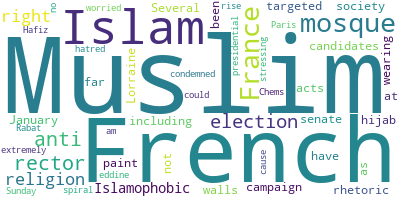
\includegraphics[scale=1]{article_1.png}
    \caption{Wordcloud d'un article de Morocco World News}
\end{figure}

\hspace{50cm}

\begin{figure}[!h]
    \centering
    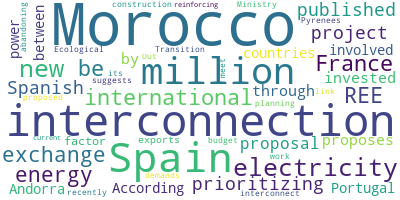
\includegraphics[scale=1]{article_2.png}
    \caption{Wordcloud d'un article de Morocco World News}
\end{figure}

\newpage

\subsection{WordCloud Français}

\vspace{20mm}

\begin{figure}[!h]
    \centering
    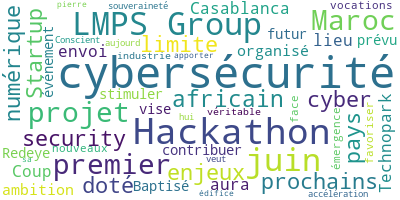
\includegraphics[scale=1]{article_3.png}
    \caption{Wordcloud d'un article de Le Matin}
\end{figure}

\begin{figure}[!h]
    \centering
    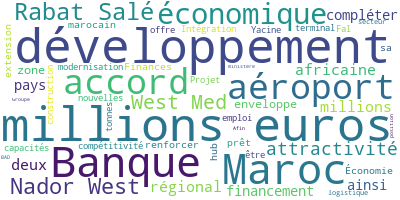
\includegraphics[scale=1]{article_4.png}
    \caption{Wordcloud d'un article de Le Matin}
\end{figure}

\newpage

\section{Topic Modeling}
\label{sec:Topic Modeling}

\subsection{Modèle non supervisé}

Le \textbf{Topic Modeling} est un modèle de machine learning \textbf{non supervisé}, c'est-à-dire qu'il ne nécessite pas d'entraînement. Les données n'étant pas étiquetées, le modèle doit donc découvrir les structures sous-jacentes à ces données de lui-même.

\subsection{Preprocessing}

On commence tout d'abord par réaliser certaines opérations sur nos données notamment la suppression des stopwords et des mots de moins de 3 lettres puis la lemmatisation après avoir supprimé les valeurs NAN. Pour ce faire ont utilisé les fonctions de la libraire \textbf{nltk}.

\subsection{Conversion}

On stocke nos données après leur nettoyage dans un dictionnaire de \textbf{gensim} pour ensuite les convertir au format \textbf{Bag Of Words} c'est-à-dire en couple mot et nombre d'occurrences où la clé est représentée par le mot et la valeur par son nombre d'occurrences.

\subsection{Application}

On applique le topic modeling à l'aide de la fonction \textbf{LdaMulticore} de \textbf{gensim} en prenant bien soin de préciser le nombre de topic à extraire du corpus, le mapping entre les identifiants des mots (entiers) et les mots (chaîne de caractères) et le nombre à effectuer d'itération dans le corpus.

\subsection{Cohérence}

Les mesures de cohérence évaluent le degré de similitude sémantique entre les mots les mieux notés dans les topics. Ces mesures aident à faire la distinction entre les topics sémantiquement interprétables et les topics dus à des inférences statistiques
Pour un bon modèle LDA la cohérence doit être comprise entre 0.4 et 0.7 au-delà et en dessous le modèle est très probablement erroné.\\

\noindent
La cohérence pour un modèle LDA est calculée en procédant aux étapes suivantes :\\

\begin{itemize}
    \item \textbf{Segmentation :} création de paires de mots à partir de sous-ensembles ;\\
    \item \textbf{Calcul des probabilités :} calcul probabilité d'occurrence d'un mot ;\\
    \item \textbf{Mesure de confirmation :} vérification « dans quelle mesure » un sous-ensemble de mots supporte un autre sous-ensemble de mots dans chaque paire ;\\
    \item \textbf{Agrégation :} agrégation de toutes les valeurs calculées à l'étape précédente en une seule valeur qui est notre score final de cohérence de sujet.
\end{itemize}

\newpage

\subsection{Résultats}

On stocke finalement les topics obtenus dans un data frame Pandas pour ensuite les garder dans un fichier csv. On peut également utiliser \textbf{pyLDAvis} pour visualiser les topics de manière interactive directement sur notre Notebook Python.\\

\begin{figure}[!h]
    \centering
    \includegraphics[scale=0.6]{topicmodel1.png}
    \caption{Topic Model Morocco World News}
\end{figure}

\hspace{100cm}

\begin{figure}[!h]
    \centering
    \includegraphics[scale=0.6]{topicmodel2.png}
    \caption{Topic Model Le Matin}
\end{figure}

\newpage

\section{Text Classification}
\label{sec:Text Classification}

\subsection{Modèle supervisé}

La classification de texte est un modèle de machine learning \textbf{supervisé}, c'est-à-dire qu'il nécessite un entraînement préalable sur des données étiquetées, le modèle doit apprendre une fonction de prédiction à partir des données annotées dont il dispose.

\subsection{Preprocessing}

On commence tout d’abord par réaliser certaines opérations sur nos données notamment la suppression des caractères spéciaux, des caractères uniques, des espaces multiples puis on convertit tout en minuscule avant d'appliquer la lemmatisation.

\subsection{Conversion}

On stocke nos données après leur nettoyage dans un \textbf{Bag Of Words}. On utilise ensuite la méthode \textbf{Term Frequency - Inverse Document Frequency} pour pouvoir pondérer l'importance d'un mot dans un document. Pour ce faire on utilise les fonctions \verb|CountVectorizer| et \verb|TfidfTransformer| de la librairie \textbf{sklearn.feature\_extraction.text}.

\subsection{K Nearest Neighbour}

Le modèle de classification des k plus proches voisins est un des modèles de classification les plus simples, il suit l'algorithme suivant :

\begin{enumerate}
    \item Sélectionner le nombre k de voisins et calculer les distances;
    \item Prendre les k voisins les plus proches selon la distance calculée;
    \item Parmi ces k voisins, compter le nombre de points appartenant à chaque catégorie;
    \item Attribuer le nouveau point à la catégorie la plus présente parmi ces k voisins.
\end{enumerate}

\begin{figure}[!h]
    \centering
    \includegraphics[scale=0.45]{KNN.jpg}
    \caption{Une itération de l'algorithme KNN}
\end{figure}

\subsection{Logistic Regression}

Un modèle de régression logistique permet aussi de prédire la probabilité qu’un événement arrive. Lorsque la valeur prédite est supérieure à un seuil, l’événement est susceptible de se produire. Pour ce faire, on utilise une fonction sigmoïde $\sigma(x) = \frac{1}{1 + \exp{-x}}$.\\

\begin{figure}[!h]
    \centering
    \includegraphics[scale=0.25]{RGL.png}
    \caption{Courbe Fonction Sigmoïde}
\end{figure}

La classification par régression logistique correspond à un simple problème d’optimisation où nous essayons d’obtenir les meilleurs paramètres $\theta$ afin que notre courbe sigmoïde $h(X) = \sigma(\theta X)$ colle le plus possible aux données d'entraînement.

\subsection{Decision Tree}

Sur un arbre de décision, chaque question correspond à un noeud. En fonction de la réponse à chaque question, nous allons nous orienter vers une branche de l’arbre pour finalement arriver sur une feuille de l’arbre qui contiendra la réponse finale.

\begin{figure}[!h]
    \centering
    \includegraphics[scale=0.6]{DecisionTree.png}
    \caption{Exemple d'arbre de décision pour la reconnaissance d'animaux}
\end{figure}

L'algorithme se demande à chaque noeud quelle feature est la plus intéressante en calculant le gain d'information. Son objectif final étant de maximiser ce gain c’est pourquoi l’arbre choisit la question qui maximise ce gain.

\subsection{Random Forest}

La forêt aléatoire est une méthode d’ensemble puisqu'elle combine plusieurs résultats pour obtenir un résultat final. Elle combine en réalité les résultats de plusieurs arbres de décision. Chaque arbre est entraîné sur un sous-ensemble aléatoirement constitué du dataset d'entraînement.\\

\begin{figure}[!h]
    \centering
    \includegraphics[scale=0.5]{RF.png}
    \caption{Forêt Aléatoire de N Arbres de Décision}
\end{figure}

Les résultats de tous les arbres de décision sont alors combinés pour donner une réponse finale. Chaque arbre “vote” et la réponse finale est celle qui a eu la majorité de votes. C'est ce qu'on appelle la méthode du \textbf{bagging}.\\

\begin{figure}[!h]
    \centering
    \includegraphics[scale=0.4]{bag.png}
    \caption{Schéma de la méthode du Bagging}
\end{figure}

\subsection{Support Vector Machine}

La classification suivant une Machine à Vecteurs de Support repose sur le tracé d'une droite qui délimite des espaces différents et constitue une réponse au problème. On cherche donc la droite qui sépare le mieux nos classes en cherchant celle dont la marge est la plus élevée. La marge étant la distance qui sépare une droite de l’observation la plus proche.\\

\begin{figure}[!h]
    \centering
    \includegraphics[scale=0.6]{SVM.png}
    \caption{Représentation du SVM}
\end{figure}

Malheureusement dans certains cas cette droite n'existe pas et le modèle n'est donc pas applicable ou alors il faut l'appliquer en omettant certaines valeurs.

\begin{figure}[!h]
    \centering
    \includegraphics[scale=0.4]{SVMM.png}
    \caption{Représentation du SVM avec une valeur extrême}
\end{figure}

\subsection{Stochastic Gradient Descent}

La Descente de Gradient est un algorithme d’optimisation qui permet de trouver le minimum de n’importe quelle fonction convexe en convergeant progressivement vers celui-ci. Dans notre cas la fonction à minimiser est la fonction de coût.\\

On part d’un point initial aléatoire puis on mesure la valeur de la pente en ce point en calculant le gradient. On progresse ensuite d’une certaine distance dans la direction de la pente qui descend.\\

Cette opération a pour résultat de modifier la valeur des paramètres de notre modèle. On répète ensuite ce processus de très nombreuses fois jusqu'à obtenir un modèle suffisamment satisfaisant.

\begin{figure}[!h]
    \centering
    \includegraphics[scale=0.5]{SGD.jpeg}
    \caption{Représentation de la descente de gradient}
\end{figure}

La descente de gradient stochastique est un type de descente de gradient qui traite un exemple d’entraînement par itération. Par conséquent, les paramètres sont mis à jour même après une itération dans laquelle un seul exemple a été traité. C’est donc plus rapide que la descente de gradient classique.

\begin{figure}[!h]
    \centering
    \includegraphics[scale=0.5]{SGD.png}
    \caption{Différence entre descente de gradient stochastique et classique}
\end{figure}

\subsection{Multi-Layer Perceptron}

\subsubsection{Réseaux neuronaux}

Le perceptron multicouche est un type de réseau neuronal artificiel à propagation directe c'est-à-dire au sein duquel l'information circule de la couche d'entrée vers la couche de sortie uniquement.\\

Le réseau se compose d'au moins trois couches de nœuds : une couche d'entrée, une couche cachée et une couche de sortie. À l'exception des nœuds d'entrée, chaque nœud est un neurone qui utilise une fonction d'activation non linéaire.

\begin{figure}[!h]
    \centering
    \includegraphics[scale=0.42]{MLP.png}
    \caption{Perceptron Multicouche}
\end{figure}

La fonction d'activation est une fonction mathématique appliquée à un signal en sortie d'un neurone artificiel. Le terme vient de l'équivalent biologique "potentiel d'activation" qui désigne le seuil de stimulation qui, une fois atteint entraîne une réponse du neurone.

\begin{figure}[!h]
    \centering
    \includegraphics[scale=0.5]{act.png}
    \caption{Fonctions d'activation}
\end{figure}

\newpage

\subsubsection{Rétro-propagation}

Le réseau utilise une technique d'apprentissage supervisée appelée \textbf{rétro-propagation}. Ses multiples couches et son activation non linéaire distinguent le réseau multicouche d'un perceptron linéaire. Il peut distinguer les données qui ne sont pas linéairement séparables.\\

La \textbf{rétro-propagation} calcule le gradient de la fonction de coût par rapport aux poids du réseau pour un seul exemple d'entrées-sorties en mettant à jour les poids pour minimiser les pertes.\\

\begin{figure}[!h]
    \centering
    \includegraphics[scale=0.7]{bp.png}
    \caption{Visualisation de la rétro-propagation}
\end{figure}

\subsection{Évaluation}

Pour évaluer la précision des modèles on va utiliser la librairie \textbf{sklearn.metrics} pour calculer le \verb|accuracy_score| qui nous donne une mesure de la précision globale de notre modèle sur les données de test.\\

On utilise aussi la fonction \verb|classification_report| qui nous donnent pour chacune des catégories de nos données les mesures suivantes :\\

\begin{itemize}
    \item \textbf{précision} : taux de prédictions positives correctes;\\
    \item \textbf{recall} : taux de positifs correctement prédits;\\
    \item \textbf{f1-score} : capacité d'un modèle à bien prédire les individus positifs.
\end{itemize}

\newpage

\subsection{Résultats Classification Report}

\begin{figure}[!h]
    \centering
    \includegraphics[scale=1]{RKNN.png}
    \caption{Classification Report K-NN}
\end{figure}

\begin{figure}[!h]
    \centering
    \includegraphics[scale=1]{RLSR.png}
    \caption{Classification Report Régression Logistique}
\end{figure}

\begin{figure}[!h]
    \centering
    \includegraphics[scale=1]{RRF.png}
    \caption{Classification Report Forêts Aléatoires}
\end{figure}

\begin{figure}[!h]
    \centering
    \includegraphics[scale=1]{CRSVM.png}
    \caption{Classification Report Support Vector Machine}
\end{figure}

\begin{figure}[!h]
    \centering
    \includegraphics[scale=1]{MSGD.png}
    \caption{Classification Report Descente de Gradient Stochastique}
\end{figure}

\begin{figure}[!h]
    \centering
    \includegraphics[scale=1]{RMLP.png}
    \caption{Classification Report Perceptron Multicouche}
\end{figure}

\clearpage

\subsection{Interprétation}

On remarque que des modèles avec quasiment le même Accuracy Score peuvent en réalité avoir des résultats assez différents sur chacune des catégories séparément. De même, on remarque que certains modèles, même avec un Accuracy Score assez bas, peuvent avoir des très bonnes précisions sur une catégorie donnée.\\

Pour avoir une meilleure idée des erreurs de nos modèles et surtout des confusions qu'il peut faire, c'est-à-dire savoir quelle catégorie il prédit lorsqu'il se trompe et avec quelle fréquence, on va utiliser les matrices de confusions. Ces mesures détaillées par catégorie permettant de rendre compte de la performance d'un modèle de classification et peuvent ensuite permettre de comprendre pourquoi le modèle se trompe afin de l'améliorer.\\

\begin{figure}[!h]
    \centering
    \includegraphics[scale=0.4]{Matrice-de-confusion.png}
    \caption{Matrice de Confusion}
\end{figure}

On peut facilement dire que la quantité de données d'entraînement joue un rôle important dans la qualité de classification. Les catégories avec peu d'articles comme \verb|politics| et \verb|society| sont les moins bien prédites contrairement à des catégories avec plus d'articles comme \verb|opinion| et \verb|education| qui sont les mieux prédits.\\

\noindent

\begin{figure}[!h]
    \centering
    \includegraphics[scale=0.6]{ACCpng.png}
    \caption{Précision des différents modèles}
\end{figure}

\clearpage

\subsection{Résultats Confusion Matrix}

\vspace{25mm}

\begin{figure}[!h]
    \centering
    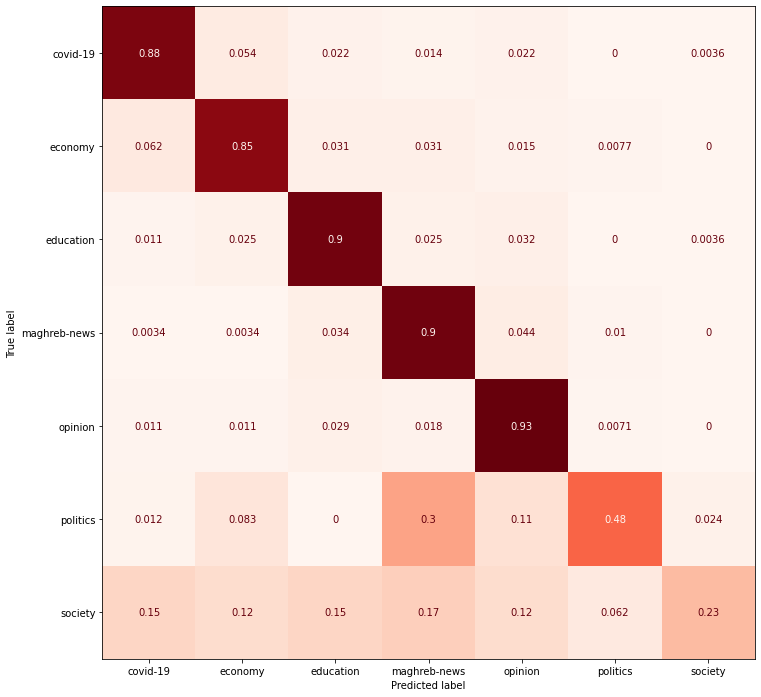
\includegraphics[scale=0.6]{LRmat.png}
    \caption{Matrice de Confusion pour la Régression Logistique}
\end{figure}

\begin{figure}[!h]
    \centering
    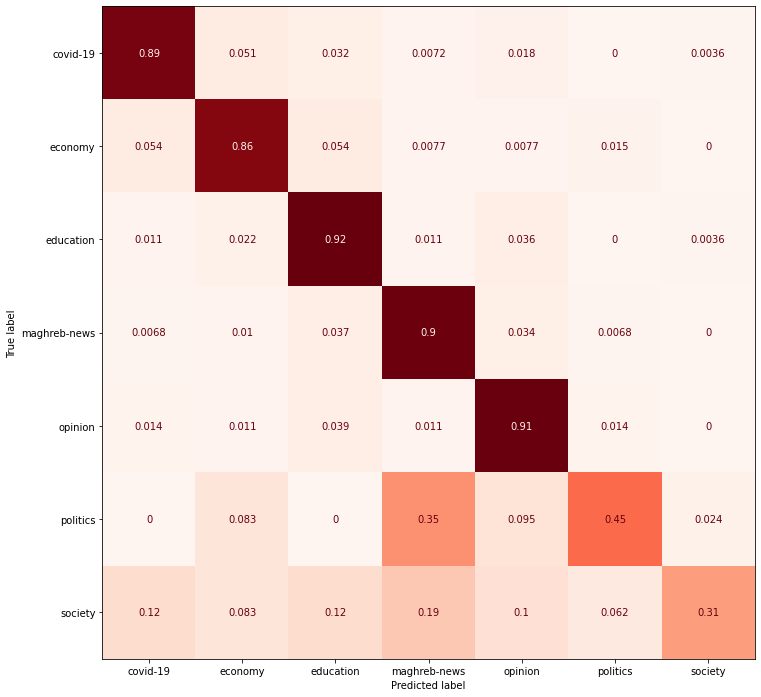
\includegraphics[scale=0.6]{SVMmat.png}
    \caption{Matrice de Confusion pour la Support Vector Machine}
\end{figure}

\begin{figure}[!h]
    \centering
    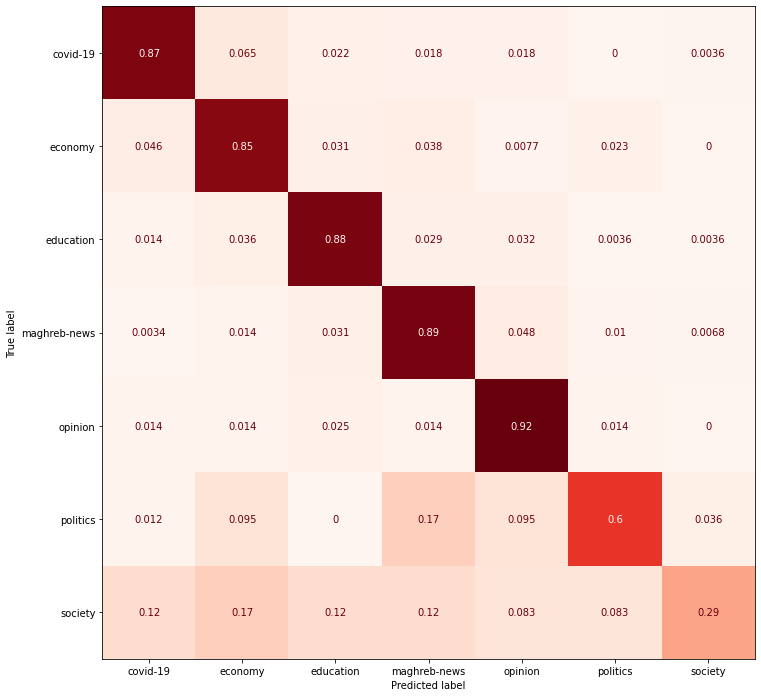
\includegraphics[scale=0.6]{SGDmat.png}
    \caption{Matrice de Confusion pour la Descente de Gradient Stochastique}
\end{figure}

\clearpage

\section{DashBoard}
\label{sec:DashBoard}

\subsection{Streamlit}

La dernière tâche de mon stage à consister en la création d'une \textbf{application web} pour présenter visuellement les résultats obtenus. Cette application web devait contenir un échantillon du data set obtenu par \verb|web scraping|, les résultats du \verb|topic modeling|, la répartition des catégories et des auteurs, les scores des différents modèles de classification et enfin les matrices de confusion des trois meilleurs modèles.\\

La librairie utilisée est \textbf{Streamlit} qui permet de transformer les scripts en applications web partageables le tout en Python sans avoir besoin de technologies front-end. La librairie est très bien documentée et propose une \emph{Cheat Sheet} très intuitive. Pour exécuter l'application il suffit d'utiliser un terminal et la commande \verb|streamlit run| :

\begin{figure}[!h]
    \centering
    \includegraphics[scale=0.55]{term.png}
    \caption{Lancement de l'application Web}
\end{figure}

Afin de pouvoir tracer des graphiques et afficher des images sur le DashBoard j'ai utilisé respectivement \textbf{Plotly} et \textbf{PIL}. De plus j'ai eu besoin de \textbf{streamlit.components} pour ajouter le code HTML obtenu avec \verb|pyLDAvis|.

\subsection{Résultat}

\begin{figure}[!h]
    \centering
    \includegraphics[scale=0.4]{Dash 1.png}
    \caption{Capture d'écran DashBoard}
\end{figure}

\begin{figure}[!h]
    \centering
    \includegraphics[scale=0.4]{Dash 2.png}
    \caption{Capture d'écran DashBoard}
\end{figure}

\begin{figure}[!h]
    \centering
    \includegraphics[scale=0.3]{Dash 3.png}
    \caption{Capture d'écran DashBoard}
\end{figure}

\begin{figure}[!h]
    \centering
    \includegraphics[scale=0.3]{Dash 4.png}
    \caption{Capture d'écran DashBoard}
\end{figure}

\begin{figure}[!h]
    \centering
    \includegraphics[scale=0.3]{Dash 5.png}
    \caption{Capture d'écran DashBoard}
\end{figure}

\clearpage

\begin{figure}[!h]
    \centering
    \includegraphics[scale=0.4]{Dash 6.png}
    \caption{Capture d'écran DashBoard}
\end{figure}

\subsection{Configuration}

D'autres librairies Python peuvent être utilisées à la place de \textbf{Streamlit} pour créer une application Web comme \textbf{Flask} ou encore \textbf{FastAPI}. Qui permettent un peu plus de liberté au niveau de la configuration que \textbf{Streamlit} :

\begin{figure}[!h]
    \centering
    \includegraphics[scale=0.8]{St 4.png}
    \caption{Fichier de configuration de Streamlit}
\end{figure}

\newpage

\section{Conclusion}
\label{sec:Conclusion}

Durant ce stage, le \emph{Web-Scraping} a permis de récupérer de manière efficace des données sur les articles de presse en ligne marocaine. L'extraction des sujets principaux des articles grâce au \emph{Topic Modeling} a donné des résultats très satisfaisants pour les articles en anglais et assez satisfaisants pour les articles en français. Enfin, la classification de texte par catégorie en utilisant différents modèles de \emph{Machine Learning} a permis d'identifier les modèles les plus efficaces pour cette tâche à savoir la \emph{Régression Logistique}, le \emph{Stochastic Gradient Descent} et le \emph{Support Vector Machine}.\\

Cependant, on se rend compte que sur certaines catégories les résultats ne sont pas satisfaisant à cause du nombre assez faible d'articles dans les données d'entraînement. Une amélioration envisageable pour la suite et la réalisation d'une campagne de \emph{Web-Scraping} massif afin de récolter une dizaine de milliers d'articles par catégories. Ensuite, une exploration plus poussée des modèles cités précédemment s'imposent afin de les paramétrer de manière à ce qu'il soit le plus efficace possible pour notre cas d'usage.\\

La suite logique pour le \emph{Haut-Commissariat au Plan} est de mettre en oeuvre à plus grande échelle toutes ces étapes en déployant une \emph{pipeline} d'extraction des données, de nettoyage, d'application du \emph{Topic Modeling} et de la \emph{Text Classification} puis du monitoring des résultats via application Web.

\begin{figure}[!h]
    \centering
    \includegraphics[scale=0.7]{pipeline.png}
    \caption{Data Pipeline}
\end{figure}

L'ensemble des missions que j'ai effectuées durant mon stage ont permis au  \emph{HCP} d'étudier la faisabilité de l'ensemble du processus, d'identifier l'ensemble des technologies nécessaires (\emph{Selenium, Nltk, Gensim, pyLDAvis, WordCloud, Plotly, Sklearn, Streamlit}) et aussi de sélectionner les modèles de \emph{Machine Learning} les plus performants.\\

Dans son optique de développement, le \emph{HCP} a effectué une refonte complète de son site mise en ligne durant mon stage le 5 juillet 2022, mes travaux rentrent en compte dans le \emph{Nouveau Modèle de Développement} puisque le numérique figure en premier lieu dans les chantiers transformateurs. J'espère que dans les mois à venir, le projet auquel j'ai participé, qui n'est encore qu'à ses balbutiements, pourra voir le jour et que la science des données se retrouvera au coeur des outils de prises de décisions.

\newpage

\section{Bibliographie}
\label{sec:Bibliographie}

~\\

\begingroup
\renewcommand{\section}[2]{}%
\begin{thebibliography}{9}

\bibitem{lamport94}
    Atindra Bandi, Medium, \textit{Web Scraping Using Selenium — Python}, \href{https://towardsdatascience.com/web-scraping-using-selenium-python-8a60f4cf40ab}{Lien vers l'article}\\
    
\bibitem{lamport94}
    Darek Tidwell, Medium, \textit{Using Selenium with Google Colaboratory}, \href{https://medium.com/@darektidwell1980/using-selenium-with-google-colaboratory-ca4a4f21021f}{Lien vers l'article}\\
    
\bibitem{lamport94}
    Baiju Muthukadan, \textit{Selenium Documentation}, \href{https://selenium-python.readthedocs.io/#}{Lien vers la documentation}\\

\bibitem{lamport94}
    Susan Li, Towards Data Science, \textit{A Complete Exploratory Data Analysis and Visualization for Text Data}, \href{https://towardsdatascience.com/a-complete-exploratory-data-analysis-and-visualization-for-text-data-29fb1b96fb6a}{Lien vers l'article}\\
    
\bibitem{lamport94}
    Michael Waskom, \textit{Seaborn Documentation}, \href{https://seaborn.pydata.org}{Lien vers la documentation}\\

\bibitem{lamport94}
    Priya Dwivedi, Towards Data Science, \textit{NLP: Extracting the main topics from your dataset using LDA in minutes}, \href{https://towardsdatascience.com/nlp-extracting-the-main-topics-from-your-dataset-using-lda-in-minutes-21486f5aa925}{Lien vers l'article}\\
    
\bibitem{lamport94}
    Susan Li, Towards Data Science, \textit{Topic Modelling in Python with NLTK and Gensim}, \href{https://towardsdatascience.com/topic-modelling-in-python-with-nltk-and-gensim-4ef03213cd21}{Lien vers l'article}\\
    
\bibitem{lamport94}
    NLTK Team, \textit{NLTK Documentation}, \href{https://www.nltk.org}{Lien vers la documentation}\\
    
\bibitem{lamport94}
    Radim Řehůřek, \textit{Gensim Documentation}, \href{https://radimrehurek.com/gensim/auto_examples/index.html#documentation}{Lien vers la documentation}\\
    
\bibitem{lamport94}
    Ben Mabey, \textit{pyLDAvis Documentation}, \href{https://pyldavis.readthedocs.io/en/latest/}{Lien vers la documentation}\\
    
\bibitem{lamport94}
    João Pedro, Towards Data Science, \textit{Understanding Topic Coherence Measures}, \href{https://towardsdatascience.com/understanding-topic-coherence-measures-4aa41339634c}{Lien vers l'article}\\
    
\bibitem{lamport94}
    Usman Malik, Stack Abuse, \textit{Text Classification with Python and Scikit-Learn}, \href{https://stackabuse.com/text-classification-with-python-and-scikit-learn/}{Lien vers l'article}\\
    
\bibitem{lamport94}
    Deepak Singh, Analytics Vidhya, \textit{Text Classification of News Articles}, \href{https://www.analyticsvidhya.com/blog/2021/12/text-classification-of-news-articles/}{Lien vers l'article}\\
    
\bibitem{lamport94}
    Scikit-Learn Team, \textit{Scikit-Learn Classification Documentation}, \href{https://scikit-learn.org/stable/supervised_learning.html#supervised-learning}{Lien vers la documentation}\\
    
\bibitem{lamport94}
    Yohan C, DataScientest, \textit{Qu’est ce que l’algorithme KNN ?}, \href{https://datascientest.com/knn}{Lien vers l'article}\\
    
\bibitem{lamport94}
    Chloé G, DataScientest, \textit{Random Forest : Forêt d’arbre de décision- Définition et fonctionnement}, \href{https://datascientest.com/random-forest-definition}{Lien vers l'article}\\
    
\bibitem{lamport94}
    Adrien R, DataScientest, \textit{La régression logistique, qu’est-ce que c’est ?}, \href{https://datascientest.com/regression-logistique-quest-ce-que-cest}{Lien vers l'article}\\
    
\bibitem{lamport94}
    Alban T, DataScientest, \textit{SVM, quoi, comment, pourquoi ?}, \href{https://datascientest.com/svm}{Lien vers l'article}\\
    
\bibitem{lamport94}
    Wikipedia, \textit{Stochastic Gradient Descent}, \href{https://en.wikipedia.org/wiki/Stochastic_gradient_descent}{Lien vers l'article}\\
    
\bibitem{lamport94}
    Wikipedia, \textit{Backpropagation}, \href{https://en.wikipedia.org/wiki/Backpropagation}{Lien vers l'article}\\
    
\bibitem{lamport94}
    Wikipedia, \textit{Multilayer Perceptron}, \href{https://en.wikipedia.org/wiki/Multilayer_perceptron}{Lien vers l'article}\\
    
\bibitem{lamport94}
    Andrew Long, Towards Data Science, \textit{Understanding Data Science Classification Metrics in Scikit-Learn in Python}, \href{https://towardsdatascience.com/understanding-data-science-classification-metrics-in-scikit-learn-in-python-3bc336865019}{Lien vers l'article}\\
    
\bibitem{lamport94}
    Sarang Narkhede, Towards Data Science, \textit{Understanding Confusion Matrix}, \href{https://towardsdatascience.com/understanding-confusion-matrix-a9ad42dcfd62}{Lien vers l'article}\\
    
\bibitem{lamport94}
    Streamlit Inc, \textit{Documentation Streamlit}, \href{https://docs.streamlit.io/library/cheatsheet}{Lien vers la Cheat Sheet}\\    
    
\bibitem{lamport94}
    Haut-Commissariat au Plan, \textit{Publications}, \href{https://www.hcp.ma/downloads/}{Lien vers les publications}\\

\bibitem{lamport94}
    Haut-Commissariat au Plan, \textit{Bases de Données Statistiques}, \href{http://bds.hcp.ma/sectors}{Lien vers les BDS}\\

\end{thebibliography}
\endgroup

\newpage

\section{Glossaire}
\label{sec:Glossaire}

~\\

\textbf{Web Scraping} : Le Web Scraping est une technique d'extraction du contenu d'un site Web via un script ou un programme dans le but de transformer les données extraites afin de les utiliser dans d'autres contextes. \textbf{Page 1}\\

\textbf{Natural Language Processing} : Le traitement du langage naturel (en français) est un domaine interdisciplinaire qui comprend la linguistique, l'informatique et l'intelligence artificielle, dans le but de développer des outils de traitement du langage naturel pour une variété d'applications. \textbf{Page 4}\\

\textbf{Topic Modeling} : En apprentissage automatique et en traitement automatique du langage naturel, un modèle thématique est un modèle probabiliste permettant de déterminer des sujets ou thèmes abstraits dans un document. \textbf{Page 4}\\

\textbf{Text Classification} : La classification et catégorisation de documents est l'activité du traitement automatique du langage naturel qui consiste à classer de façon automatique des ressources documentaires. Ainsi la classification peut se faire par genre, par thème, ou encore par opinion. \textbf{Page 4}\\

\textbf{Bases de Données Statistiques} : Une base de données statistiques est une base de données classique qui retourne uniquement des informations et des données statistiques aux requêtes des utilisateurs, en fonction des enregistrements qui sont utilisée à des fins d'analyse statistique. \textbf{Page 7}\\

\textbf{Latent Dirichlet Allocation} : Dans le domaine du traitement automatique du langage naturel, l’allocation de Dirichlet latente est un modèle génératif probabiliste permettant d’expliquer des ensembles d’observations définis par des similarités de données par le moyen de groupes non observés. \textbf{Page 9}\\

\textbf{Natural Language Toolkit} : Développée par Steven Bird et Edward Loper du département informatique de l'Université de Pennsylvanie, la boîte à outils de traitement du langage naturel est une bibliothèque de logiciels Python pour le traitement automatique du langage. \textbf{Page 11}\\

\textbf{Preprocessing} : La manipulation ou à la suppression de données avant qu'elles ne soient utilisées afin d'assurer ou d'améliorer les performances, il constitue une étape importante dans le processus d'exploration de données. Son résultat est l'ensemble des données d'entraînement et de test. \textbf{Page 19}\\

\textbf{DashBoard} : Tableau de bord en français, est un outil permettant la visualisation de données de manière interactive ou non en faisant appel à différentes représentations visuelles, différents indicateurs et différentes hiérarchisations des données. \textbf{Page 26}\\

\newpage

\section{Annexes}
\label{sec:Annexes}

\subsection{Développement Durable et Responsabilité Sociétale}

Dans une optique de responsabilité sociétale et environnementale le HCP s'est engagé sur plusieurs fronts. Il s'est donc doté d'une plateforme \href{http://plateforme-odd.hcp.ma/ODD_HCP/fr/}{ODD} spécialement conçu pour avoir un suivi de l'avancée de ces objectifs avec différents indicateurs basés sur des données disponibles pour tous.\\

\begin{figure}[!h]
    \centering
    \includegraphics[scale=0.59]{ODD.png}
    \caption{Capture d'écran du site ODD de l'HCP}
\end{figure}\\

En plus de mener ses propres études en interne, le HCP fournit aux différents organismes nationaux ainsi qu'aux bureaux d'études internationaux des données fiables et des indicateurs précis pour pouvoir mener leurs études autour de ses différents objectifs.\\

\begin{figure}[!h]
    \centering
    \includegraphics[scale=0.43]{oddz.png}
    \caption{Capture d'écran du site ODD de l'HCP}
\end{figure}

\newpage

La plateforme \href{http://plateforme-odd.hcp.ma/ODD_HCP/fr/}{ODD} de suivi des objectifs de développement durable comprend 17 objectifs principaux distincts à différents horizons qui sont les suivants :\\

\begin{enumerate}
    \item Éliminer la pauvreté sous toutes ses formes et partout dans le monde
    \item Éliminer la faim, assurer la sécurité alimentaire, améliorer la nutrition et promouvoir l’agriculture durable
    \item Permettre à tous de vivre en bonne santé et promouvoir le bien-être de tous à tout âge
    \item Assurer à tous une éducation équitable, inclusive et de qualité et des possibilités d’apprentissage tout au long de la vie
    \item Parvenir à l’égalité des sexes et autonomiser toutes les femmes et les filles
    \item Garantir l’accès de tous à des services d’alimentation en eau et d’assainissement gérés de façon durable
    \item Garantir l’accès de tous à des services énergétiques fiables, durables et modernes, à un coût abordable
    \item Promouvoir une croissance économique soutenue, partagée et durable, le plein emploi productif et un travail décent pour tous
    \item Bâtir une infrastructure résiliente, promouvoir une industrialisation durable qui profite à tous et encourager l’innovation
    \item Réduire les inégalités dans les pays et d’un pays à l’autre
    \item Faire en sorte que les villes et les établissements humains soient ouverts à tous, sûrs, résilients et durables
    \item Établir des modes de consommation et de production durables
    \item Prendre d’urgence des mesures pour lutter contre les changements climatiques et leurs répercussions
    \item Conserver et exploiter de manière durable les océans, les mers et les ressources marines aux fins du développement durable
    \item Préserver et restaurer les écosystèmes terrestres, en veillant à les exploiter de façon durable, gérer durablement les forêts, lutter contre la désertification, enrayer et inverser le processus de dégradation des terres et mettre fin à l’appauvrissement de la biodiversité
    \item Promouvoir l’avènement de sociétés pacifiques et inclusives aux fins du développement durable, assurer l’accès de tous à la justice et mettre en place, à tous les niveaux, des institutions efficaces, responsables et ouvertes à tous
    \item Renforcer les moyens de mettre en œuvre le Partenariat mondial pour le développement durable et le revitaliser
\end{enumerate}

\hspace{1cm}

À ce sujet, le HCP a publié deux rapports nationaux sur les objectifs du développement durable au Maroc. Ils sont tous les deux téléchargeables aux liens suivants :\\

\href{https://odd.hcp.ma/file/232819/}{Rapport National 2021 : Les objectifs du développement durable au Maroc dans le contexte de la Covid-19 (Version française)}\\

\href{https://odd.hcp.ma/file/218058/}{Rapport National 2020 sur la mise en oeuvre par le Royaume du Maroc des Objectifs de Développement Durable (Version Française)}

\subsection{Annexe A : Extrait Code Web Scraping}

\vspace{30mm}

\begin{figure}[!h]
    \centering
    \includegraphics[scale=1]{setup ws.png}
\end{figure}

\hspace{100cm}

\begin{figure}[!h]
    \centering
    \includegraphics[scale=1]{recup link.png}
\end{figure}

\begin{figure}[!h]
    \centering
    \includegraphics[scale=1]{scrap art.png}
\end{figure}

\clearpage

\subsection{Annexe B : Extrait Code WordCloud}

\begin{figure}[!h]
    \centering
    \includegraphics[scale=1]{WCnet.png}
\end{figure}

\begin{figure}[!h]
    \centering
    \includegraphics[scale=0.9]{WCC.png}
\end{figure}

\clearpage

\subsection{Annexe C : Extrait Code Topic Modeling}

\begin{figure}[!h]
    \centering
    \includegraphics[scale=0.75]{lda1.png}
\end{figure}

\begin{figure}[!h]
    \centering
    \includegraphics[scale=1]{lda2.png}
\end{figure}

\begin{figure}[!h]
    \centering
    \includegraphics[scale=0.9]{lda3.png}
\end{figure}

\begin{figure}[!h]
    \centering
    \includegraphics[scale=0.9]{lda4.png}
\end{figure}

\begin{figure}[!h]
    \centering
    \includegraphics[scale=0.9]{lda5.png}
\end{figure}

\begin{figure}[!h]
    \centering
    \includegraphics[scale=0.85]{lda61.png}
\end{figure}

\begin{figure}[!h]
    \centering
    \includegraphics[scale=0.8]{lda7.png}
\end{figure}

\begin{figure}[!h]
    \centering
    \includegraphics[scale=0.8]{lda8.png}
\end{figure}

\begin{figure}[!h]
    \centering
    \includegraphics[scale=0.9]{lda9.png}
\end{figure}

\clearpage

\subsection{Annexe D : Extrait Code Text Classification}

\vspace{20mm}

\begin{figure}[!h]
    \centering
    \includegraphics[scale=1]{TC1.png}
\end{figure}

\begin{figure}[!h]
    \centering
    \includegraphics[scale=1]{TC2.png}
\end{figure}

\begin{figure}[!h]
    \centering
    \includegraphics[scale=1]{TC3.png}
\end{figure}

\begin{figure}[!h]
    \centering
    \includegraphics[scale=0.8]{TC4.png}
\end{figure}

\begin{figure}[!h]
    \centering
    \includegraphics[scale=1]{TC8.png}
\end{figure}

\begin{figure}[!h]
    \centering
    \includegraphics[scale=1]{TC7.png}
\end{figure}

\begin{figure}[!h]
    \centering
    \includegraphics[scale=1]{TC5.png}
\end{figure}

\begin{figure}[!h]
    \centering
    \includegraphics[scale=1]{TC6.png}
\end{figure}

\begin{figure}[!h]
    \centering
    \includegraphics[scale=1]{TC9.png}
\end{figure}

\begin{figure}[!h]
    \centering
    \includegraphics[scale=1]{TC10.png}
\end{figure}

\begin{figure}[!h]
    \centering
    \includegraphics[scale=1]{TC11.png}
\end{figure}

\clearpage

\subsection{Annexe E : Extrait Code DashBoard}

\vspace{20mm}

\begin{figure}[!h]
    \centering
    \includegraphics[scale=0.9]{St 1.png}
\end{figure}

\begin{figure}[!h]
    \centering
    \includegraphics[scale=0.95]{St 2.png}
\end{figure}

\begin{figure}[!h]
    \centering
    \includegraphics[scale=0.8]{St 3.png}
\end{figure}

\end{document}
